% !TeX spellcheck = es_ES
\documentclass[12pt, titlepage]{article}
\usepackage[utf8]{inputenc}
\usepackage[spanish]{babel}
\usepackage{float}
\usepackage[letterpaper, margin=2.5cm]{geometry}
\usepackage[nottoc,notlot,notlof]{tocbibind} % Hace que se agregen las referencias al indice
\usepackage{url}
\usepackage{graphicx} 
\usepackage{listings}
\usepackage{color}
\definecolor{dkgreen}{rgb}{0,0.6,0}
\definecolor{gray}{rgb}{0.5,0.5,0.5}
\definecolor{mauve}{RGB}{253,151,31}

\lstset{frame=tb,
    language=Sql,
    aboveskip=3mm,
    belowskip=3mm,
    showstringspaces=false,
    columns=flexible,
    basicstyle={\small\ttfamily},
    numbers=none,
    numberstyle=\tiny\color{gray},
    keywordstyle=\color{blue},
    commentstyle=\color{dkgreen},
    stringstyle=\color{mauve},
    breaklines=true,
    breakatwhitespace=true,
    tabsize=2,
    morekeywords={use}
}

\title{Tarea 2}
\author{Carlos Tonatihu Barrera Pérez \\ Profesor: Hernández Contreras Euler \\ Bases de Datos \\ Grupo: 2CM1 }
\date{27 de marzo de 2017}

\begin{document}
	\maketitle
	\tableofcontents
	\section{Introducción}
	El modelo Entidad-Relación es un es una herramienta fundamental para diseñar esquemas que posteriormente se implementaran en un gestor de bases de datos. Este modelo se representa a través de diagramas y está formado por varios elementos, los más importantes son las entidades, atributos y relaciones.\cite{LIBRO}
	
	\begin{figure}[H]
		\begin{center}
			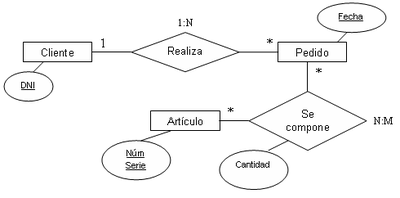
\includegraphics[width=12cm, height=4cm]{img/modelo.png}
			\caption{Ejemplo del modelo ER.}
			\label{fig:hasta-use}
		\end{center}
	\end{figure}
	
	El primer elemento que conforma el modelo entidad relación son las entidades las cuales representan cosas u objetos (ya sean reales o abstractos), que se diferencian claramente entre sí. Estas entidades se representan en un diagrama con un rectángulo, como los siguientes.
	
	\begin{figure}[H]
		\begin{center}
			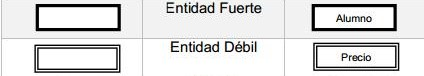
\includegraphics[width=10cm, height=2cm]{img/entidad1.jpg}
			\caption{Entidades del modelo ER.}
			\label{fig:hasta-use1}
		\end{center}
	\end{figure}
	
	También existen los atributos los cuales definen o identifican las características de la entidad (dicho de otro modo es el contenido de esta entidad). Cada entidad contiene distintos atributos, que dan información sobre esta entidad. Estos atributos se representan como elipses unidos a las entidades con el nombre del atributo dentro.\cite{WEB}
	
	\begin{figure}[H]
		\begin{center}
			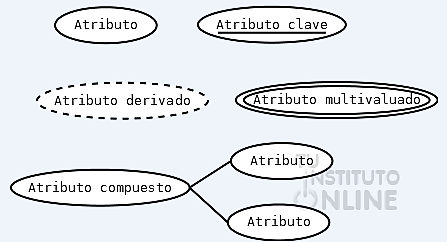
\includegraphics[width=10cm, height=4cm]{img/atributo.png}
			\caption{Tipos de atributos en el diagrama entidad relación.}
			\label{fig:hasta-use2}
		\end{center}
	\end{figure}
	
	Por ultimo las relaciones son un vínculo que nos permite definir una dependencia entre varias entidades, es decir, nos permite exigir que varias entidades compartan ciertos atributos de forma indispensable. Las relaciones se muestran en los diagramas como rombos, que se unen a las entidades mediante líneas.
	\begin{figure}[H]
		\begin{center}
			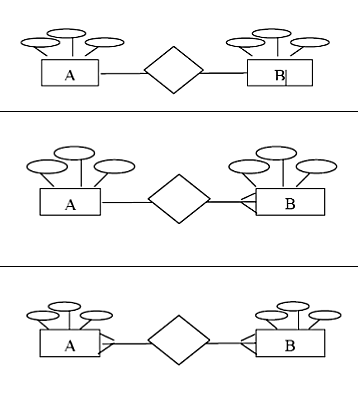
\includegraphics[width=10cm, height=10cm]{img/relaciones.png}
			\caption{Representación de las relaciones 1 a 1, 1 a muchos y muchos a muchos.}
			\label{fig:hasta-use3}
		\end{center}
	\end{figure}
\newpage
	\section{Desarrollo}
	Para esta tarea fueron modelados los siguientes diagramas.
	\subsection{GYM}
	\begin{figure}[H]
		\begin{center}
			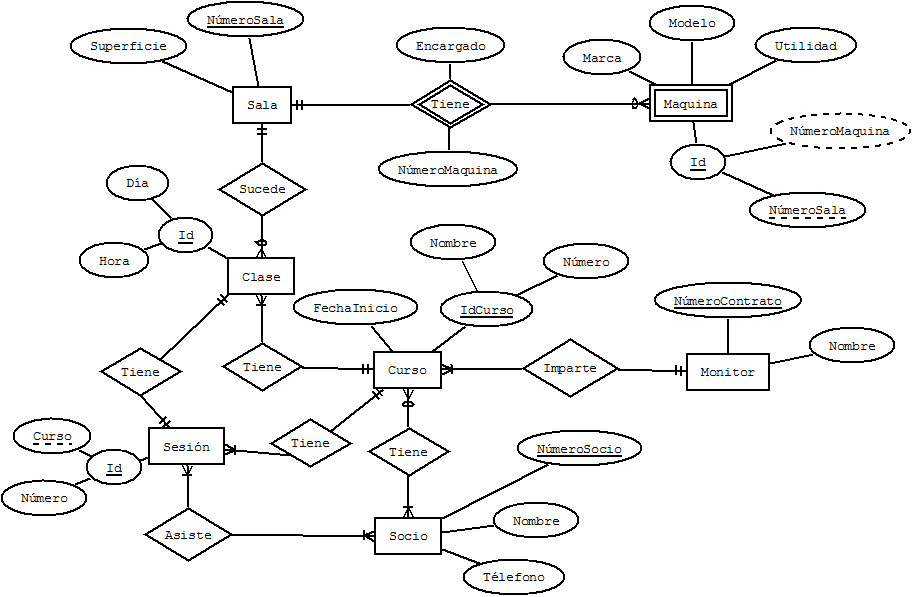
\includegraphics[width=16cm, height=14cm]{img/Gym.png}
			\label{fig:hasta-use4}
		\end{center}
	\end{figure}
	\subsection{Metro}
	\begin{figure}[H]
		\begin{center}
			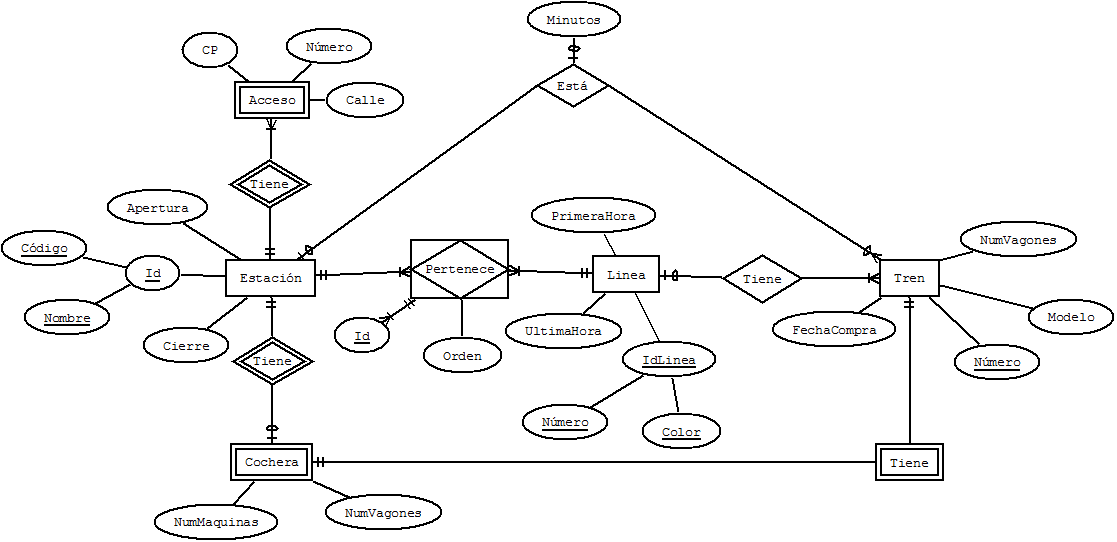
\includegraphics[width=16cm, height=12cm]{img/Metro.png}
			\label{fig:hasta-use5}
		\end{center}
	\end{figure}
	\subsection{Elecciones}
	\begin{figure}[H]
		\begin{center}
			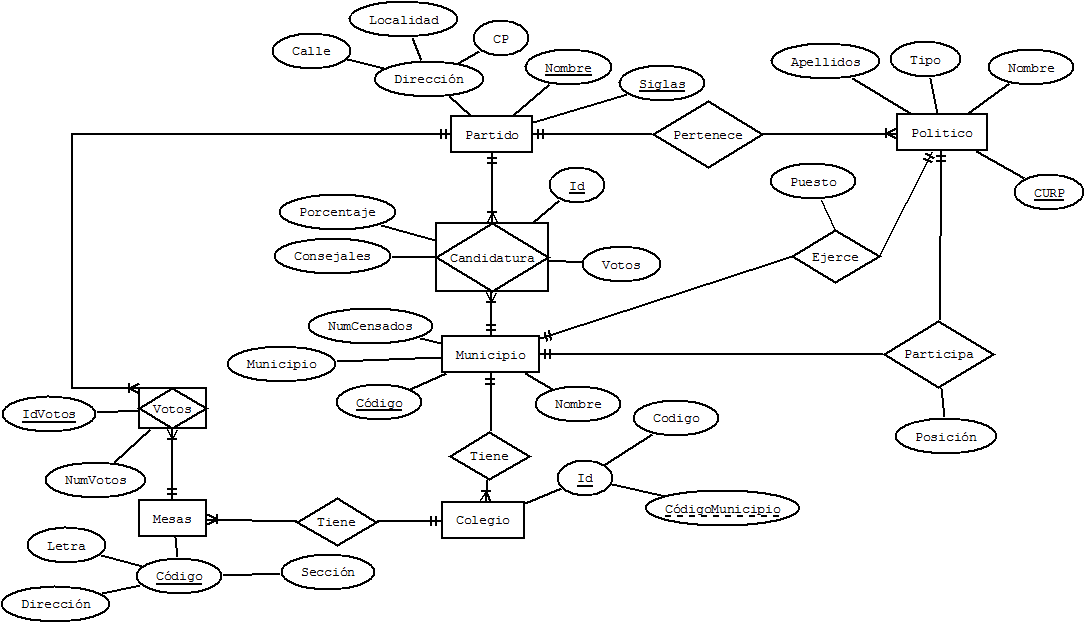
\includegraphics[width=16cm, height=12cm]{img/Elecciones.png}
			\label{fig:hasta-use6}
		\end{center}
	\end{figure}
	\subsection{Farmacias}
	\begin{figure}[H]
		\begin{center}
			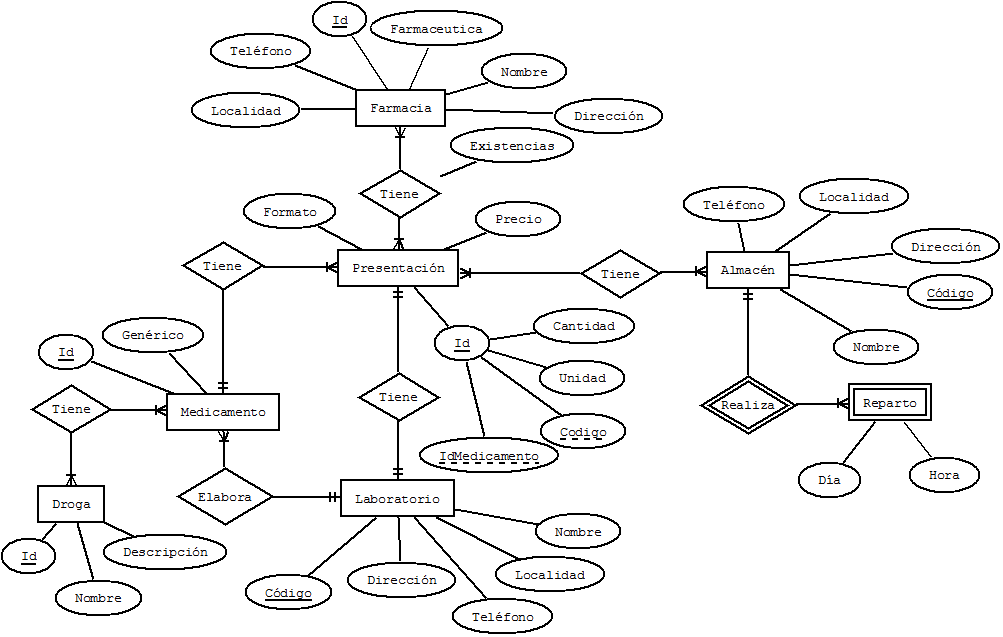
\includegraphics[width=16cm, height=14cm]{img/Farmacia.png}
			\label{fig:hasta-us3}
		\end{center}
	\end{figure}
	\subsection{Patentes}
	\begin{figure}[H]
		\begin{center}
			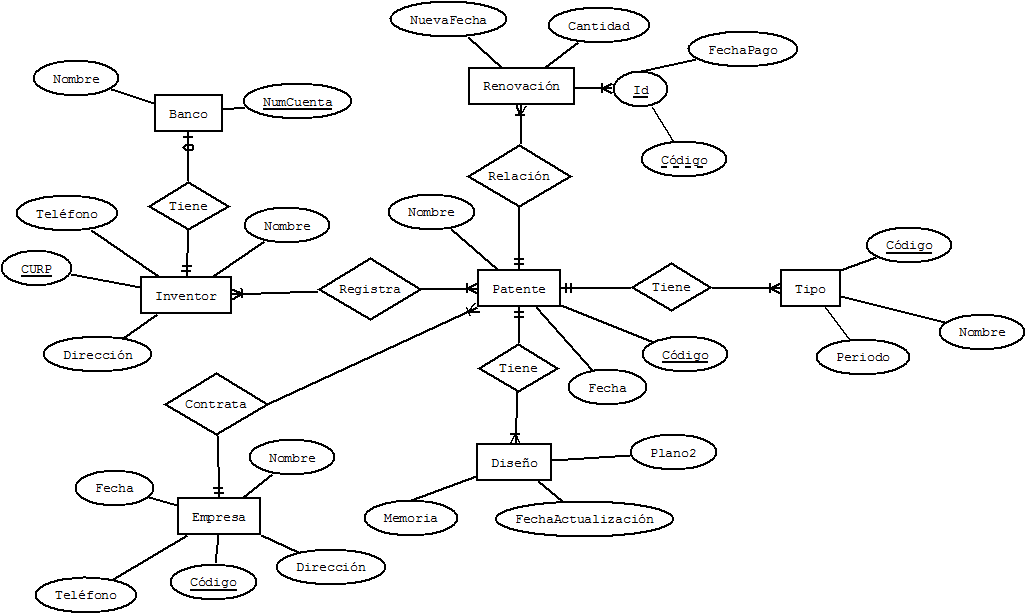
\includegraphics[width=16cm, height=13cm]{img/Patentes.png}
			\caption{Modelo ER.}
			\label{fig:hasta-3}
		\end{center}
	\end{figure}
	\subsection{Conciertos}
	\begin{figure}[H]
		\begin{center}
			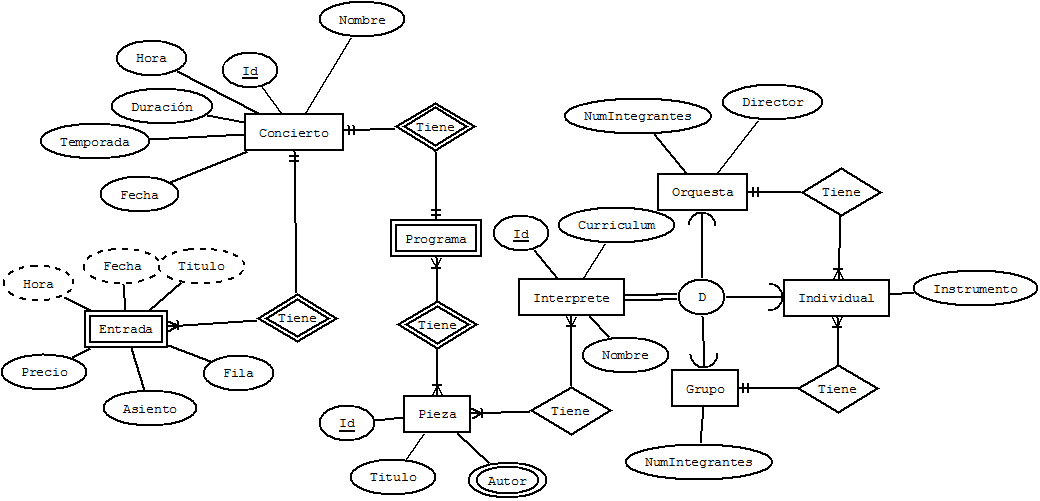
\includegraphics[width=16cm, height=10cm]{img/Conciertos.png}
			\caption{Modelo entidad-relación.}
			\label{fig:hastause3}
		\end{center}
	\end{figure}
	\section{Conclusiones}
	Estos ejercicios fueron bastante laboriosos de realizar de una forma lo más adecuada a las restricciones que contenía el problema. Existen varios puntos que pueden ser mejorados con ayuda de normalización para poder lograr una mejor integridad que la realizada en estos diagramas entidad-relación que al final se vería reflejada en el modelo relacional. Además, se puede dar el caso en el que un mismo problema pueda ser resuelto de diferentes formas cada una con sus ventajas y desventajas. 
	\bibliography{bibliografia} 
	\bibliographystyle{ieeetr}
\end{document}]
